\documentclass[12pt]{article}
\usepackage[french]{babel}
\usepackage[T1]{fontenc}
\usepackage[utf8]{inputenc}
\usepackage{graphicx}
\usepackage{eurosym}
\usepackage {times}
\usepackage{fancyhdr}
\usepackage{bm}
\usepackage{listings}
\title{Projet CamlT'OCR par SMK \\ Rapport de dernière soutenance}
\pagestyle{fancyplain} \lhead{\textit{Projet CamelT'OCR}} \rhead{\textit{SMK}}
\date{11-12-2013}
\author{
  Timothe \textit{Tim-Tim} Bureau-Godart(bureau\_t) \and
  Leopold \textit{Meta} Szabatura (szabat\_l) \and
  Louis \textit{Zab} Forget (forget\_l) \and
  Maxime \textit{Kylox} Gaudron (gaudro\_m)
1      }

\begin{document}
\maketitle
\newpage
\tableofcontents
\newpage
\section{Introduction}
\subsection{presentation des membres}
\subsubsection{Louis "\textit{Zab}" Forget}
J'ai toujours etais tres curieux, au point de partir souvent dans tous les sens. J'ai toujours voulu savoir comment marchent les pages webs. C'est dans cette optique que j'ai appris a faire du HTML et CSS en troisieme. J'ai ensuite voulu savoir comment marchent les jeux videos, puis divers programmes. Il y a quelques jours je me suis demandais commemt marchent les gps qui indiquent la densite du traffic.
\subsubsection{Timothe "\textit{Tim-Tim}" Bureau Godart}
Je n'étais encore qu'un gosse quand le drame s'est produit, une attaque de livre dans ma propre maison ! J'étais dépassé, tous ses mots sans définition, tous ses paragraphes sans résumé, j'allais sombrer dans un univers d'horreur et d'épouvante sans pouvoir en ressortir... Quand soudain, la lumière apparu, elle avait la forme d'une gameboy géante et me sauva de l'enfer des livres. Depuis ce jour je lui voue un culte sans précédent et cherche à percer tous ses mystères.
Très jeune, je possédais déjà mon propre ordinateur, construis par un ami de mes parent, dès lors je n'ai jamais acheté d'ordinateur, je les ai toujours eu en pièce détaché. Cependant je ne m'intéressais pas trop a la programmation bien que cela me titillais un peu de ne pas savoir comment mes personnages de jeux vidéo pouvais attaquer sur la simple pression d'un bouton (car oui, je suis un grand fan de jeu vidéo et j'ai commencé très petit, ce qui est vite devenu une grande passion). J'ai commencé a réellement m'intéresser à cette univers en classe de seconde, grâce à l'option MPI. Je me suis documenté sur plusieurs langages quand j'ai entendu parler d'EPITA, ce qui m'a donné un but, faire partie de cette école pour faire de ma passion mon métier.
\subsubsection{Leopold "\textit{Meta}" Szabatura}
Je me suis intéressé à l'informatique à l’âge de 15 ans.
C'est pendant cette année de seconde que, en fouillant sur ma calculatrice, j'ai découvert l'univers fantastique de la programmation.
Cela m'a rapidement mené sur la voix du java ou je faisais mes premiers pas dans le monde de la programmation oriente objet.
\subsubsection{Maxime "\textit{kylox}" Gaudron}
J'ai toujours vécu dans un monde plus ou moin informatisé. Adepte de tout les petits appareils electroniques et mecaniques. A tel point que je démontais tout et que plus rien ne marchait ! Je me suis donc mis naturellement à aller chercher un peu plus loin dans le fonctionement interne des appareils. L'ocr est donc pour moi un grand apprentissage et une decouverte qui permet d'envisager differente possibilite de reconnaissance et de systemes automatisé !
\section{L'interface graphique}

\section{Site Internet}
Pour commencer, vous pouvez trouver notre site web à l'adresse suivante : cmalt-ocr.epiproject.eu.\\
Pour ce site, nous avons décidé de faire une interface simple, épuré et pas très rechercher pour facilité la navigation. Pour cela, nous avons utilisé du HTML/CSS et du PHP. Notre site est hébergé sur le serveur de de Louis Forget.\\
Le site internet n'est pas une partie principale du projet, il passe souvent au second plan à cause des difficultés rencontré au cours du projet. Cependant, nous avons fait en sorte que notre site ne soit pas délaissé.

\subsection{HTML/CSS}
La base de notre site repose sur le language HTML (HyperText Markup Language) qui gère et organise le contenu. Vous direz par exemple : « Ceci est mon titre, ceci est mon menu, voici le texte principal de la page, voici une image à afficher, etc. » et il vous l'afichera dans une page comme indiqué dans votre code. Cependant, il ne fera qu'afficher, sans aucun style ni mise en page, des paragraphes et des titres écrit en noir sur fond blanc. C'est là qu'intervient le CSS (Cascading Style Sheets, aussi appelées Feuilles de style) qui va révlutionner la page que vous êtes en train de créer. Le rôle du CSS est de gérer l'apparence de la page (agencement, positionnement, décoration, couleurs, taille du texte…) Ce qui va donner une ame à votre site (sauf s'il est roux, mais j'en doute...).\\

C'est ainsi que notre site a vu le jour, mais il a falu l'amélioré, et la, un autre problème s'est posé, comme chaque page du site a le même squelette, modifier une toute petite partie de celui ci revient à modifier à la main chaque page du site, ce qui n'est pas très sypatique pour aller vite. Mais nous avons trouvé la solution, nous avons introduit du PHP dans notre code !

\subsection{PHP}
Le PHP est un langage que seuls les serveurs comprennent et qui permet de rendre les sites dynamiques. C'est PHP qui « génère » la page web. Une de ces principals fonction est de "se souvenir" des bouts de code (c'est pas pour rien que c'est un éléphant). En effet, pour que notre site est le même squelette sur toute ses pages, nous allons écrire un squelette dans un fichier et nous utiliserons une balise PHP pour le "charger" dans toute les page de notre site. Grâce à se procédé miraculeux, nous pouvons modifier le squelette du site tout entier en ne modifiant qu'un seul fichier. Bien enttendu notre site ne comporte pas beaucoup de pages, mais nous utilisons cette methode pour éviter les pages anciennes au milieu des nouvelles.


\begin{figure}[h]
  \begin{center}
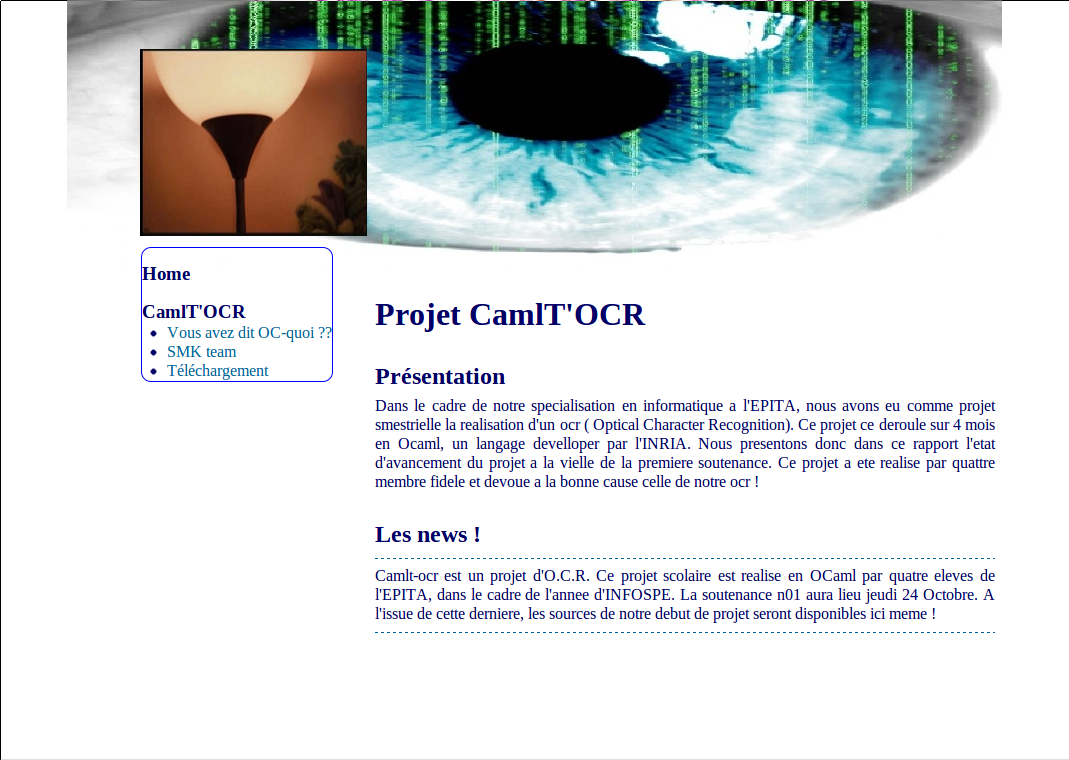
\includegraphics[width=0.50\textwidth]{site.png}
\caption{la page principale du site internet}
\end{center}
\end{figure}
\section{Le prè-traitement}
\subsection{Le niveau de gris}
\textbf{Le concept}:\\
Une image se compose d'élément appelé pixel et definie par trois composante (en realite quattres mais ceci est une autre histoire) qui sont R,G et B correspondant au valeur Red, Green et Blue d'un pixel. Cette etape est primordiale car elle va permettre le bon traitement de l'image par l'ensemble des étapes aui la succède.\\
\textbf{La realisation}:\\
Pour réaliser ce niveau de gris on va travailler sur les trois composantes d'un pixel et appliquer la fromule suivante :
\\
\begin{center}
	\[x = \frac{0.299 \times R + 0.587 \times G + 0.114 \times B}{3}\]
\end{center}
à l'ensemble des pixels de l'image. Le niveau de gris est operationel dans notre ocr, nous pouvons donc passer à la tache suivante.
\begin{figure}[h]
	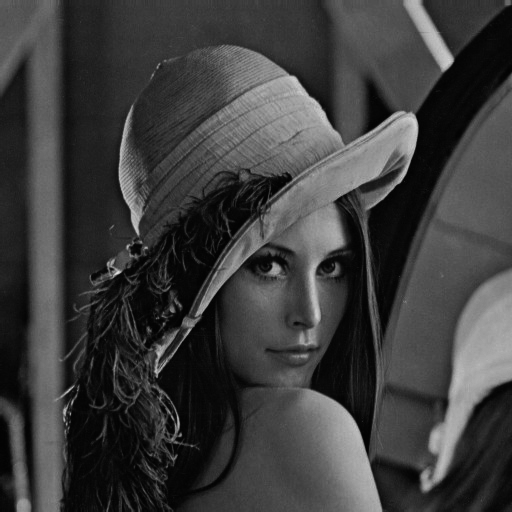
\includegraphics[width=0.50\textwidth]{grey.png}
	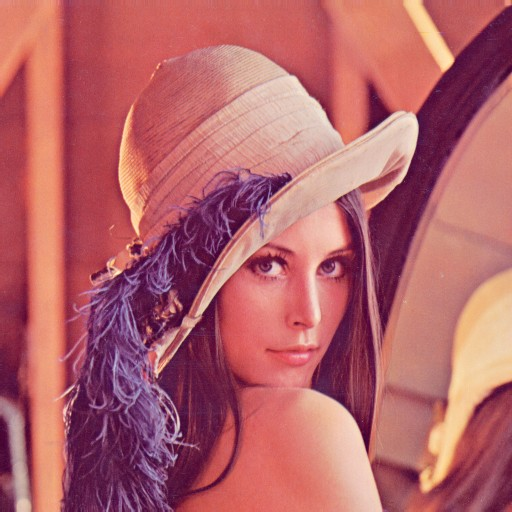
\includegraphics[width=0.50\textwidth]{lena.jpg}
	\caption{avec et sans nuance (captain obvious is obvious)}
\end{figure}
\newpage
\subsection{Le filtre median}
\textbf{Le concept}:\\
Le filtre median va pour chaque pixels de l'image recuperer le triplet (R,G,B) de chaque pixel autour du pixel traitré et trier ces pixels par ordre croissant. Il suffit juste de recuperer la valeur mediane de la liste trier. Le passe dans cette algo et qyue l'on doit passer les pixels sur une autre image pour pas fausser les calculs sur la premiere image !
\vspace{0.8cm}
\textbf{La realisation}:\\
En pratique ce filtre ne s'applique pas sur toute les images car sinon elle floute l'image et la rend intraitable. Je suis actuellement en recherche d'un algorithme permettant de palier ce gros probleme. Au niveau aulgoritemiaue on obtiens
\vspace{0.8cm}
\begin{figure}[h]
	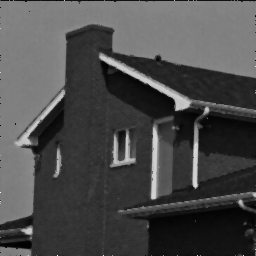
\includegraphics[width=0.50\textwidth]{house.png}
	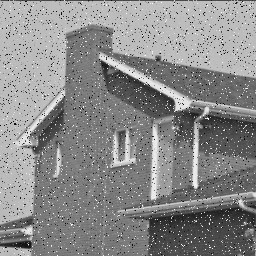
\includegraphics[width=0.50\textwidth]{house.jpg}
	\caption{presentation du filtre median}
\end{figure}
\newpage
\subsection{La binarisation}
\textbf{Le concept}:
Nous utilisons l'algorithme d'Otsu, du nom de son inventeur Nobuyuki Otsu. Qui se base sur l'histogramme d'un image. L'histogramme est un tableau de 255 element, ici des entiers, qui represente le nombre d'occurence d'un niveau de gris ( les niveau de gris allant de 0 (blanc) a 255 (noir). Dans un permier temps va creer un tableau pour y mettre les valeur traiter de l'histogramme de la maniere suivante
\begin{center}
	\[ p_{i} = \frac{h_{i}} {width * height}\]
\end{center}
qui renvoie la population du niveau de gris i dans l'ensemble des pixels de l'image.
Nous allons ensuite traiter tout les pixels de l'image en fonction de ce tableau et de deux autres formules magique ! qui sont pour un pixel k :\\
\begin{minipage}[h]{5cm}
	\begin{lstlisting}
	v = 0;
	for i = 0 to k do
	v = v + h.(i) * i
	done
	return v
	\end{lstlisting}
\end{minipage}
\begin{minipage}[h]{5cm}
	\begin{lstlisting}
	m = 0
	for i = 0 to k do
	m = m +. h.(i) * i
	done
	return m
	\end{lstlisting}
\end{minipage}
\vspace{0.8cm}
\\Le tout est injecter dans la formule

\[ s = v(i,p) \times (1 - v(i,p) \times (p.(255)) \times v(i,p) - m(i,p))^{2}\]
La methode de binarisation est plutot au point nous obtenons de tres bon resultats !
\begin{figure}[h]
	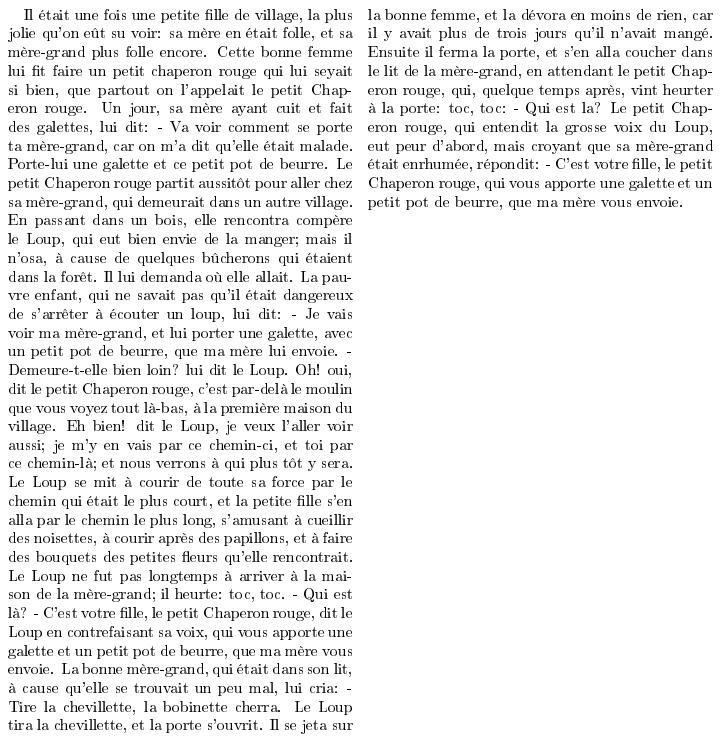
\includegraphics[width=0.50\textwidth]{bin.png}
	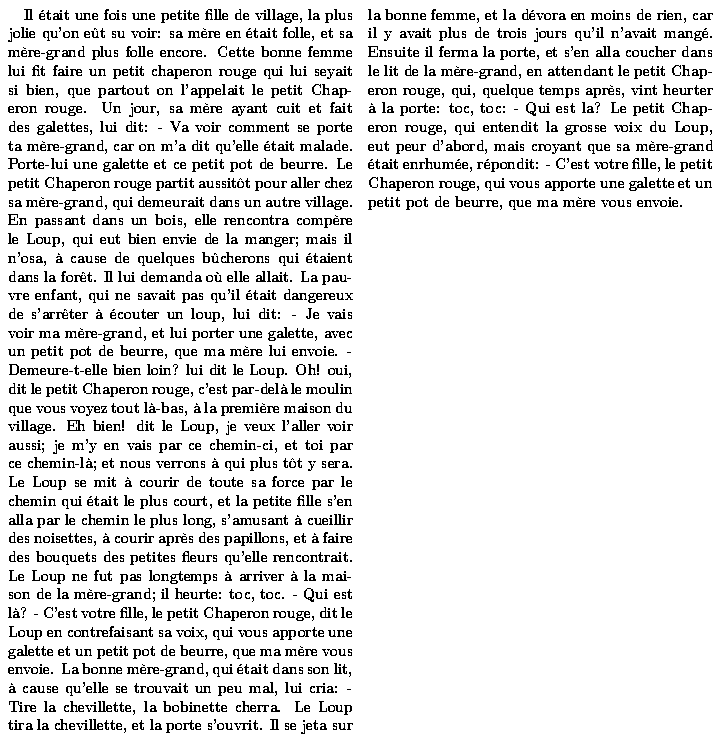
\includegraphics[width=0.50\textwidth]{bin2.png}
	\caption{exemple de binarisation}
\end{figure}

\subsection{la rotation d'image}
\subsubsection{Détection d'angle}
Je me suis donc occupe de la transformation de Hough. La transforme de hough est une techmiaue de reconnaissance de formes invente en 1962 par Paul Hough.
Le principe qui sous-tend la transforme de Hough est qu'il existe un nombre infini de ligne passant par un point dont la seule difference est l'orientation (l'angle). La transforme generalise de Houg fonctionne sur le principe qu'une droite peux s'ecrire sous la forme
\[r = x\cos{\theta}+y\sin{\theta}\]
A chaque pixels noir on essaye de trouver la vlauer maximum de r. Cette valeur represente la droite qui alligne le plus de pixel noir. On la retiens et on vote dans un tableau pour son angle associer. On recommence sur tout les pixels. L'angle qui a recu le plus de vote estl'anlge de rotation de l'image( minore de la moitier de l'intervalle pour pouvoir faire ressortir les angles negatifs).
\\
\newpage
Voici le principe de l'algo en pseudo code :
\begin{lstlisting}
for y =0 to hauteur de l'image do
for x =0 to largeur de l'image do
if (pixel noir ) then
angle = -Pi/2
while (angle < Pi/2) do
begin
r = x*cos(angle)+y*sin(angle)
if(r>o) then
/* increment tableau de vote */
angle ++
end
end
done
done

\end{lstlisting}

\begin{figure}[h]
	\centering
	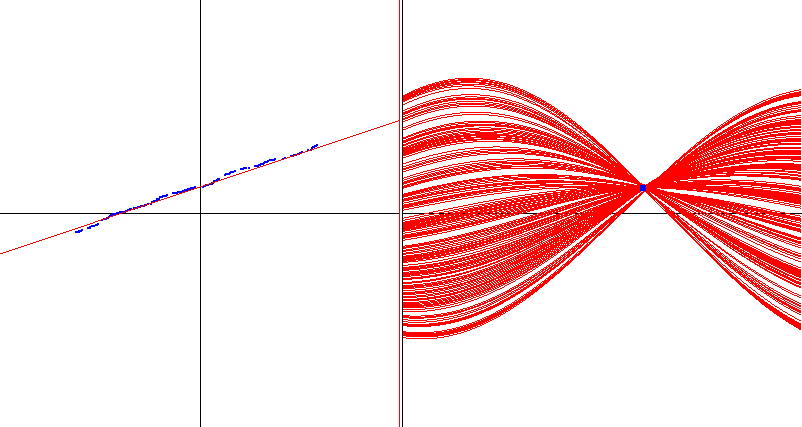
\includegraphics[width=0.80\textwidth]{hough.png}
\end{figure}
\newpage
\subsection{La rotation}
La rotation est effectue grace a une matrice de rotation. La methode consiste a assosicie chaque pixel (i, j) a une matrice [|[|i|]; [|j|]|] puis d'utilliser la formule suivate :
\\
\[A_{i,j}R_{\theta} = A'_{i,j} avec R = [|[|cos \theta; -sin \theta|]; [|sin \theta; cos \theta|]|] \]
\\
Le resultat sera alors de la forme [|[|i'|]; [|j'|]|], il faut alors creer une image d'une (diag, diag) avec diag la diagonal de l'image source, puis assigne la couleur du pixel (i, j) au pixel (i', j').
\subsection{Decoupage de l'image}
Le decoupage de l'image s'effectue en deux etapes, la premiere est de creer deux histogrammes, l'un representant le nombre de pixel noir sur sur chaque colonne et l'autre sur chaque ligne. Puis nous allons analyser chaque histogramme separement, l'histogramme va etre parcouru, et si le contenu est plus eleve qu'un certain seuil, la case sera considerer comme du texte, des premiers blocks vont donc etre forme, une fois ces blocks formees l'algorithme est reappele mais cette fois avec le deuxieme histogramme ce qui a pour effet de redecouper les blocks et d'enlever de plus en plus de parties blanches. Le processus est appele recursivement jusqu'a ce que les blocks aient la taille d'un charactere.
\subsection{Redimensionement de l'image }
Le redimensionement de l'image est utile pour pouvoir normaliser les caracteres a mettre en entre du reseau de neurone.En effet,toutes les entres du reseau de neurone doivent etre identique.Il est evident que tous les caracteres detecte par l'algorithme de XY-cut n'ont pas la meme taille.Il faut donc mettre a la meme taille tous les caracteres.Il existe plusieurs methode complexe et d'autre moins complexe mais qui provoquent souvent une baisse de la qualite de l'image.J'ai donc utilise une methode intermediaire : l'interpolation bilineaire.
Enfaite c'est assez simple, dans un premier temps on cree un ratio de largeur (x ratio = largeur de notre image/largeur attendue ) et un ratio de hauteur (y ratio= hauteur de l'image/hauteur attendue). On va cree une matrice correspondant a l'image de destination.A chaque image pixel de coodonne (x,y) de l'image attendue on va attribue les pixels de coordonne (x*x ratio,y * y ratio) de l'image source.
Voici l'algorithme en pseudo code :
\begin{lstlisting}
algorithme zoome (image src , entiers (w1,h2 )) /* dimension image attendue */
Debut
  image dst
  entier x_ratio = src.largeur/w2;
  entier y_ratio = src.hauteur/h2;
  pour x=0  a h2-1 faire
    pour y=0 a w2-1 faire
      dst(x,y) <-src(x_ratio*x,y_ratio*y);
    fin  pour
  fin pour
retourne dst; 
\end{lstlisting}
le probleme  est qu'avec cet algorithme nous creons ce qu'on appel de l'aliasing :
\begin{figure}[h]
    \centering
    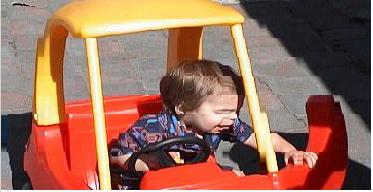
\includegraphics[width =0.80\textwidth]{aliasing.jpg}
\end{figure}
C'est a dire un trop grand contraste de couleur entre les differents pixels.Visuellement il apparait une forme d'escalier de gros contraste qui degrade fortement l'image. Le probleme de la qualite de l'image n'en est pas vraiment un pour nous.En effet nous travaillons sur des images binarises donc l aliasing cree des contrastes de blanc et de noir , ce qui a pour effet de parfois grossir certaines lettres.Ce probleme est a nouveau regle par le fait que l'on met en entre du reseau de neurone, uniquement le countoure des lettres (filtre laplacien) :
\begin{figure}[h]
    \centering
    
\includegraphics[width =0.80\textwidth]{ABCD.jpg}
\end{figure}


\section{Les filtres de convolution}

\section{Le post-traitement}

\section{le réseau de neurones}
Nous avons le regret d'annoncer que notre reseau de neuronne n'est pas fonctionel
néanmoins nous avons fait pas mal de recherche la dessus. Tout abords qu'est ce qu'un neurone ? 
\subsection{un neurone}
un neurone, en biologie, se compose de plusieur partie, nous allons nous contenter aux plus simples c'est à dire : l'axone et le noyau. l'axone est le lien qui permettra de relier plusieur neurone entre eux et le noyaux son centre de commande la ou se fera l'action du neurone. Notre reseau de neurone vas donc simuler le fonctionnement d'un neurone.
\subsection{un peu d'histoire}
Les reseau de neurone et autre perceptron sont une science a multiple facette qui a connu de nombreux retournement de situation. Ils naissent en 1950 de deux neurologues : Warren McCulloch et Walter Pitts.
\subsection{ce que compose notre reseau de neurone}
\subsubsection{le neurone}
Nous allons donc simuler un neurone formel par : 
\begin{itemize}
\item un poids 
\item une valeur 0 ou 1 
\item un seuil
\end{itemize}
Le poids sera la "niveau" de notre neurone c'est lui qui decidera si le neurone va être actif ou non, il pêse (jeux de mot) vraiment dans le réseau de neurone.\\
Sa valeur 0 ou 1 nous travaillons en flottant pour une meilleur valeur de comparaison avec son seuil et sa valeur quand on la passe dans notre fonction sigmoïde (que nous verrons un peu plus loin.\\
Et finallement son seuil qui determinera si le neroune vaux 1 ou 0. Le poids sera comparer à la sigmoïde de 
\subsubsection{la fonction d'activation}
Pour un reseau de neurone il existe plusieur fonction d'activation qui sont :
\begin{itemize}
\item sigmoïde
\item tangente hyperboliqe
\item Heaviside
\end{itemize}
\vspace{0.5cm}
Nous avons choisis d'implementer la fonction sigmoïde car plus partique pour la méthode d'apprentissage par retropropagation.
Mais faisons tout de même un bref tour d'horizon pour justifer ce choix :
\begin{itemize}
\item
La fonction Heaviside est une fonction discontinue tel que :
\begin{center}
$
 \forall x \in R, H(x) =  \left \{
\right \{
 $
\end{center}
La fonction n'est pas dérivable est pose donc un porblème.
\item
La fonction tangente hyperbolique caractériser par :
\begin{center}
\[ th(x) = \frac{e^{x} - e^{-x}}{e^{x} + e^{-x}}\]
\end{center}
\item
Mais nous avons choisis la fonction sigmoïde qui se "rapproche" un peu de la tangente hyperbolique mais la dérivé est nettement plus simple et plus facile à manier que la tangente hyperbolique. La fonction sigmoïde est representé par :
\begin{center}
\[ f(x) = \frac{1}{1 + e^{-x}} \]
\end{center}
L'avantage majeur de cette fonction est qu'elle utilisé en porbabilité logistique et permet de repartir equitablement l'ensemble des poids concernés car l'esperence d'obtenir la moyenne est de 0, ce qui correspond a un équité entre toute les valeurs de poids de notre reseau de neurone dans une couche donné.
Deplus sa dérivé est facilement calculable et vaux
\begin{center}
\[ f(x) = \frac{e^{-x}}{1+e^{-x}} \]
\end{center}
Nous verrons a quoi sert sa dérivé par la suite.
\end{itemize}

\subsubsection{la fonction de seuil}
Une fois nous avons appliquer notre sigmoïde sur les poids menant a un pixel on test si le resultat est superieur au seuil de notre neurone qui est choisis aléatoirement.
Si le resultat depasse le seuil alors le neurone vaut 1 sinon il vaut 0.

\subsection{Algorithmique}
Passon a la mise en pratique de toute ces formules.
L'algorithme prend en paramètre une matrice qui represente un caractère. Donc une matrice de 9x9 (choix arbitraire).
 Notre réseau de neurone possède ainsi 81 entrées. Nous appliquons donc chaque cellule de notre matrice a une entré de notre reseau de neurone.
Nous initialisons l'ensemble des neurones du réseau a 0 et un poids tiré au hasard, car comme chacun sait tout le monde ne démarre pas ave le même cerveau.
C'est alors que la magie opère, nous allons calculer la valeur de chaque neurone de la couche suivante a partir des poids et des valeurs des neurones précédants.
\[ x_{i} = g(\sum_{j} x_{j} w_{ji}) \]
$x_{i}$ est la valeur de neurone i dans la couche suivante\\
$g$ la fonction sigmoïde\\
$x_{j}$ la valeur du neurone j dans la couche \\
$w_{ij}$ le poids qui permet de passer du neurone $x_{j}$ à $x_{i}$\\

On obtien donc pour chaque neurone $x_{i}$ une valeur que l'on va comparé avec le seuil de ce même neurone pour savoir si on va le mettre à 1 ou a 0. On répète ainsi cette action sur toutes les couches jusqu'à la derniere.
\\
Mais comment cela fonctionne-t-il ? C'est alors que pour la deuxieme fois la magie opère. Car nous voulons reconnaitre des inputs pour en tirer un résultat. C'est alors qu'arrive la rétropogation de l'érreur.

\subsection{l'apprentissage}

Il existe plusieurs types d'apprentissage et nous avons choisis la rétropropagation de l'erreur.
Nous allons donc faire apprendre des motifs a notre réseau de neurone. Pour cela on va lui faire faire un apprentissage.
 Notre algorithme va prendre en paramètre un état initial défini et un état final, celui qui doit correspondre à  l'état inital.
Nous allons parcourir le réseau de neurone comme vu précédament et ainsi obtenir une sortie. 
Nous comparons alors notre sortie à notre état final voulu.
Deux choix s'offre à nous : ils sont égaux et alors la c'est gagné ! ca veux dire que les poids sont bien équilibré pour reconnaitre notre motif d'entré.
Sinon on part pour un rééquilibrage des poids. A ce moment la entre en scène notre charmante dérivé de fonctoin sigmoïde qui va nous premettre de faire varier les poids (dérivé... variation... variation.. dérivé... ca ne fait rire que moi...).
Tot d'abord nous calculons l'erreur sur la dernière couche grâce a :
\[e_{i} = g'(\sum_{i}w_{ji}x_{i})(s_{i}-y_{i})\]
$s_{i}$ la valeur du neurone i sur notre sortie voulue\\
$y_{i}$ la valeur du neurone i sur notre sortie obtenue\\
$w_{ij}$ le poids entre le neurone i et son prédéceseur j\\
$x_{i}$ la valeur de notre neutrone i sur la couche actuel\\
$e_{i}$ l'erreur commise.
Et nous pouvons ainsi rétropopagé cette erreur et mettre à jour les poids grâce a\[e_{j} = g'(\sum_{j} x_{j} w_{ji})\sum_{i}w_{ij}e_{i}\]
$e_{j}$ l'erreur sur la couche suivante 
$g'$ la dérivé de la fonction sigmoïde
$x_{j}$ la valeur du neurone j sur la couche précédante
$w_{ij}$ le poid entre le neurone j de la couche précédante et du neurone i de la couche courante
$e_{i}$ l'erreur sur la couche courante.

Une fois que l'on a calculer les différentes érreurs on peut mettre a jour les poids 
\[ w_{ij} = w_{ij} - \lambda e_{i} x_{j}\]
$e_{i}$ l'erreur sur la couche 
$\lambda$ le coefficient d'apprentissage comprise entre 0 et 1 
$x_{j}$ la valeur du neurone j sur la couche precedante.

C'est alors que tou les poids rééquilibrer on peut rélancer un parcours de notre reseau de neurone avec les même paramètre et recommence la retropropagation tant que la couche de sortie n'est pas égale à la couche désiré.

Voila l'apprentissage pour une valeur. Pour plusieure on prend une batterie de test et on la lance jusqu'à ce que tout les test soit concluant les un après les autres.

\subsection{ce qui ne marche pas avec notre réseau de neurone}
L'apprentissage ne se déroule pas bien, impossible de vraiment savoir pourquoi peut être un problème de sur-apprentissage...


\section{Le correcteur orthographique}
Nous aurions pus utiliser sur le texte le correcteur orthographique de GTK mais nous nous sommes quand meme interesser a la correction orthographique suivant deux methodes 
\subsection{La distance de levenshtein}
La distanve de levenshtein se base sur la difference de suppresion addition et substitution de lettre entre deux mots. Cette methode se base sur le calcul d'une matrice entre les deux mots.
\subsection{Soundex}


\end{document}
